\renewcommand*{\arraystretch}{1.1}

\subsection*{BI / read / 1}
\label{section:bi-read-01}

% change \emph{} to use sans-serif font
\let\oldemph\emph
\renewcommand{\emph}[1]{{\footnotesize \sf #1}}

\renewcommand{\currentQueryCard}{1}
\marginpar{
	\raggedleft
	\vspace{0.22ex}

	\queryRefCard{bi-read-01}{BI}{1}\\
	\queryRefCard{bi-read-02}{BI}{2}\\
	\queryRefCard{bi-read-03}{BI}{3}\\
	\queryRefCard{bi-read-04}{BI}{4}\\
	\queryRefCard{bi-read-05}{BI}{5}\\
	\queryRefCard{bi-read-06}{BI}{6}\\
	\queryRefCard{bi-read-07}{BI}{7}\\
	\queryRefCard{bi-read-08}{BI}{8}\\
	\queryRefCard{bi-read-09}{BI}{9}\\
	\queryRefCard{bi-read-10}{BI}{10}\\
	\queryRefCard{bi-read-11}{BI}{11}\\
	\queryRefCard{bi-read-12}{BI}{12}\\
	\queryRefCard{bi-read-13}{BI}{13}\\
	\queryRefCard{bi-read-14}{BI}{14}\\
	\queryRefCard{bi-read-15}{BI}{15}\\
	\queryRefCard{bi-read-16}{BI}{16}\\
	\queryRefCard{bi-read-17}{BI}{17}\\
	\queryRefCard{bi-read-18}{BI}{18}\\
	\queryRefCard{bi-read-19}{BI}{19}\\
	\queryRefCard{bi-read-20}{BI}{20}\\
	\queryRefCard{bi-read-21}{BI}{21}\\
	\queryRefCard{bi-read-22}{BI}{22}\\
	\queryRefCard{bi-read-23}{BI}{23}\\
	\queryRefCard{bi-read-24}{BI}{24}\\
	\queryRefCard{bi-read-25}{BI}{25}\\
}



\noindent\begin{tabularx}{\queryCardWidth}{|>{\queryPropertyCell}p{\queryPropertyCellWidth}|X|}
	\hline
	query & BI / read / 1 \\ \hline
%
	title & Posting summary \\ \hline
%
	pattern & \multicolumn{1}{c|}{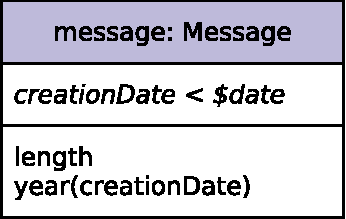
\includegraphics[scale=\patternscale,margin=0cm .2cm]{patterns/bi-read-01}} \\ \hline
%
	desc. & Given a date, find all \emph{Messages} created before that date. Group
them by a 3-level grouping:

\begin{enumerate}
\def\labelenumi{\arabic{enumi}.}
\tightlist
\item
  by year of creation
\item
  for each year, group into \emph{Message} types: is \emph{Comment} or
  not
\item
  for each year-type group, split into four groups based on length of
  their content

  \begin{itemize}
  \tightlist
  \item
    \texttt{0}: 0 \textless{}= length \textless{} 40~(short)
  \item
    \texttt{1}: 40 \textless{}= length \textless{} 80~(one liner)
  \item
    \texttt{2}: 80 \textless{}= length \textless{} 160~(tweet)
  \item
    \texttt{3}: 160 \textless{}= length~(long)
  \end{itemize}
\end{enumerate}
 \\ \hline
%
	
		params &
		\innerCardVSpace{\begin{tabularx}{\attributeCardWidth}{|>{\paramNumberCell}c|>{\varNameCell}M|>{\typeCell}m{\typeWidth}|Y|} \hline
		$\mathsf{1}$ & date
 & Date
 &  \\ \hline
		\end{tabularx}}\innerCardVSpace \\ \hline
	
%
	
		result &
		\innerCardVSpace{\begin{tabularx}{\attributeCardWidth}{|>{\resultNumberCell}c|>{\varNameCell}M|>{\typeCell}m{\typeWidth}|>{\resultOriginCell}c|Y|} \hline
		$\mathsf{1}$ & year & 32-bit Integer & R &
				Year of the \emph{Message}
 \\ \hline
		$\mathsf{2}$ & isComment & Boolean & M &
				\texttt{true} for \emph{Comments}, \texttt{false} for \emph{Posts}
 \\ \hline
		$\mathsf{3}$ & lengthCategory & String & C &
				\texttt{0} for short, \texttt{1} for one-liner, \texttt{2} for tweet,
\texttt{3} for long
 \\ \hline
		$\mathsf{4}$ & messageCount & 32-bit Integer & A &
				Total number of \emph{Messages} in that group
 \\ \hline
		$\mathsf{5}$ & averageMessageLength & 32-bit Integer & A &
				Average length of the \emph{Message} content in that group
 \\ \hline
		$\mathsf{6}$ & sumMessageLength & 32-bit Integer & A &
				Sum of all \emph{Message} content lengths
 \\ \hline
		$\mathsf{7}$ & percentageOfMessages & 32-bit Float & A &
				Number of \emph{Messages} in group as a percentage of all messages
created before the given date
 \\ \hline
		\end{tabularx}}\innerCardVSpace \\ \hline
	
%
	
		sort		&
		\innerCardVSpace{\begin{tabularx}{\attributeCardWidth}{|>{\sortNumberCell}c|>{\varNameCell}M|>{\directionCell}c|Y|} \hline
		$\mathsf{1}$ & year
 & $\desc
$ &  \\ \hline
		$\mathsf{2}$ & isComment
 & $\asc
$ & \texttt{false\ \textless{}\ true}, i.e.~the ordering puts \emph{Posts}
first, and \emph{Comments} second
 \\ \hline
		$\mathsf{3}$ & lengthCategory
 & $\asc
$ & order based on the length of the category, \texttt{0} (short),
\texttt{1} (one liner), etc.
 \\ \hline
		\end{tabularx}}\innerCardVSpace \\ \hline
	%
	%
	CPs &
	\multicolumn{1}{>{\raggedright}l|}{
		\chokePoint{1.2}, 
		\chokePoint{3.2}, 
		\chokePoint{4.1}, 
		\chokePoint{8.1}, 
		\chokePoint{8.2}, 
		\chokePoint{8.3}, 
		\chokePoint{8.4}, 
		\chokePoint{8.5}, 
		\chokePoint{8.6}, 
		\chokePoint{8.7}, 
		\chokePoint{8.8}, 
		\chokePoint{8.9}
		} \\ \hline
	%
	%
\end{tabularx}
\queryCardVSpace

% change \emph back to the old one
\renewcommand{\emph}[1]{\oldemph{#1}}